\documentclass[aspectratio=169,xcolor=dvipsnames]{beamer}
\beamertemplatenavigationsymbolsempty
\usepackage[normalem]{ulem}
\usepackage{comp2402}
\usepackage{xmpmulti}
\renewcommand{\emph}[1]{{\itshape\color{blue}#1}}
\newcommand{\emphen}[1]{{\itshape #1}}
\title{Interfaces/Abstract Data Types}
\author{COMP2402}
\date{}

\begin{document}

\begin{frame}
  \titlepage
\end{frame}

\begin{frame}
  \frametitle{Interfaces/Abstract Data Types}
 
  \begin{itemize}
   \item<+->Describes what a data structure \emph{does}:
     \begin{itemize}
        \item<+->supported operations (the \emph{interface})
        \item<+->meaning of operations (the \emph{semantics})
     \end{itemize}
   \item<+-> \sout{Representation and implementation}
        \end{itemize}
\end{frame}

\begin{frame}
  \frametitle{Abstract Data Types/Interfaces}

   B. Liskov and S. N. Zilles, Programming with Abstract Data Types, \emph{SIGPlan Notices}, 9(4), pp. 50-59, 1974.\\
  \begin{center}
   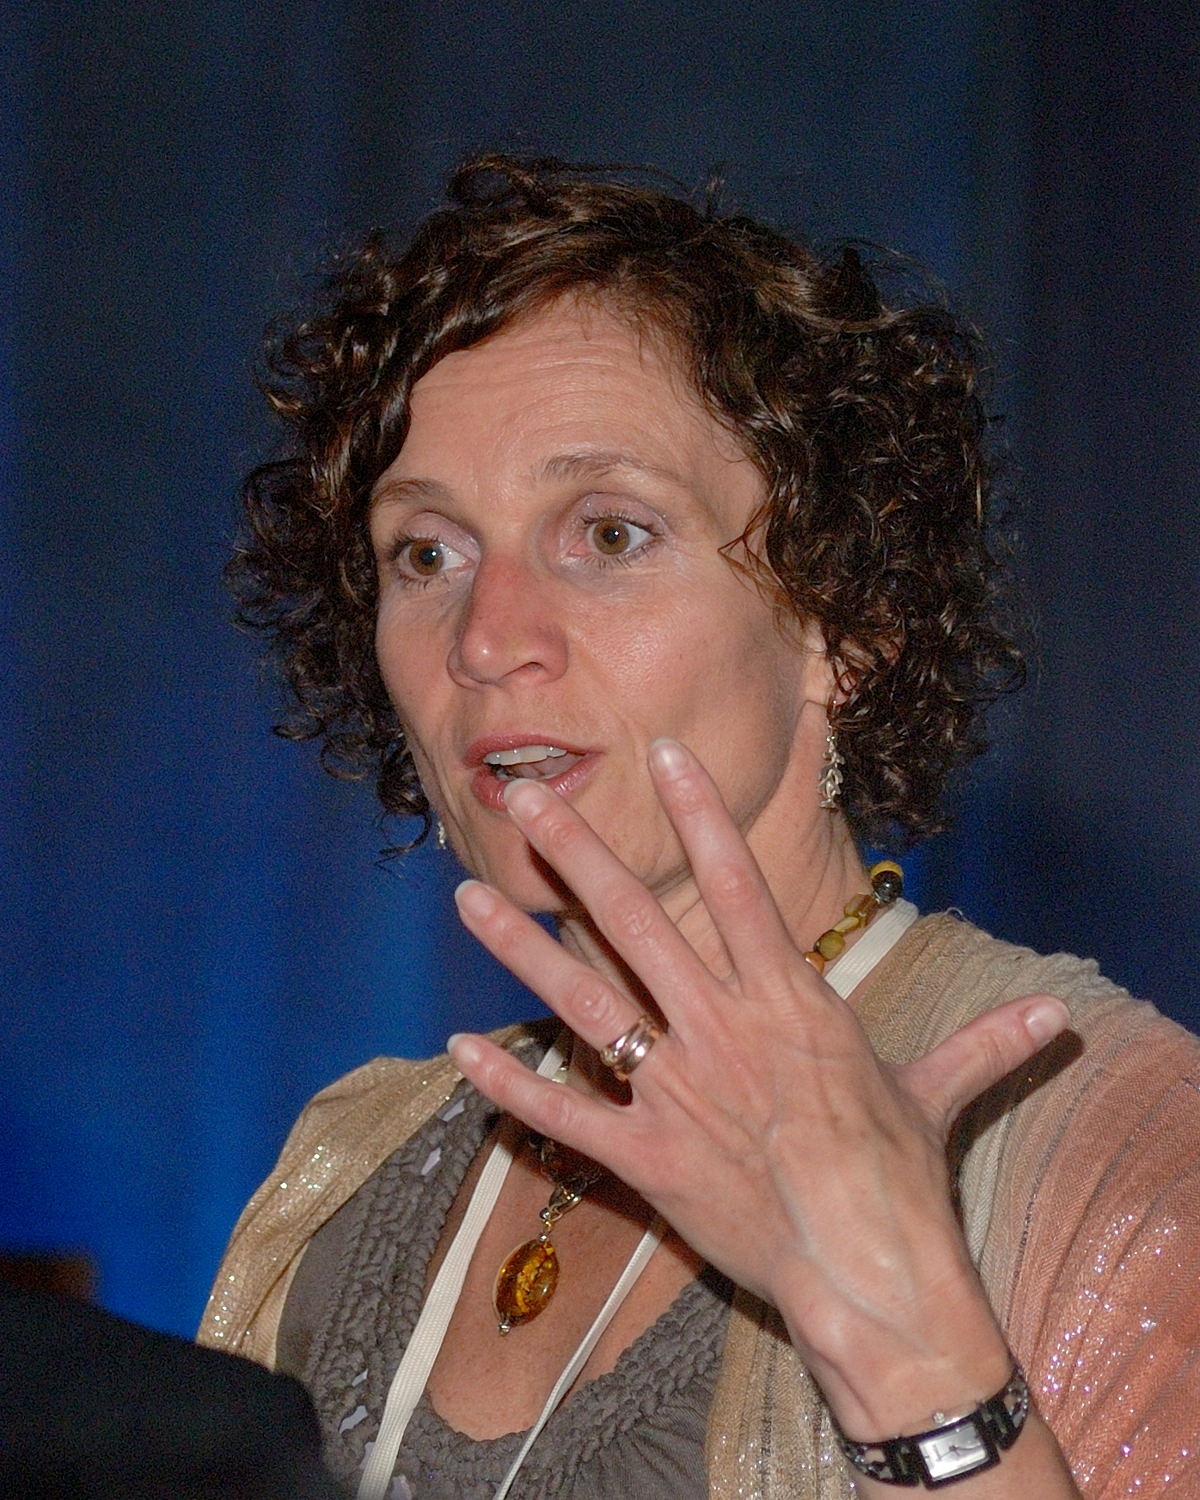
\includegraphics[height=.6\textheight]{images/liskov}\\
   B.~Liskov at the Turing Centenary Celebration (Wikimedia commons)
  \end{center}
\end{frame}

\begin{frame}
\title{The List Interface}
\maketitle
\end{frame}


\begin{frame}
  %\transdissolve[duration=0.05]
  \frametitle{List}
  \framesubtitle{A sequence of elements}
 
  \begin{itemize}
    \item<1-> Operations: \only<3->{#size()#}%
                        \only<4->{, #get(i)#}%
                        \only<5->{, #set(i,x)#}%
                        \only<6->{, #add(i,x)#}%
                        \only<7->{, #remove(x)#}
  \end{itemize}
     \begin{center}
      \only<1>{\includegraphics{figs/list-1}}%
      \only<2-7>{\includegraphics{figs/list-2}}%
      \only<8->{\multiinclude[<+>][format=pdf,start=1]{figs/list}}
     \end{center}

\end{frame}

\begin{frame}
\title{The USet (Unordered Set) Interface}
\maketitle
\end{frame}


\begin{frame}
  \frametitle{USet}
  \framesubtitle{An \emphen{unordered} collection of \emphen{distinct} items}
  \begin{itemize}
    \item<+-> Operations: \only<4->{#size()#}%
                        \only<5->{, #add(x)#}%
                        \only<6->{, #remove(x)#}%
                        \only<7->{, #find(x)#}%
  \end{itemize}
     \begin{center}
      \only<1-6>{\includegraphics{figs/uset-1}}%
      \only<7->{\multiinclude[<+>][format=pdf,start=1]{figs/uset}}
     \end{center}

\end{frame}

\begin{frame}
  \frametitle{Map}
  \framesubtitle{Another Kind of USet}
 
  \begin{itemize}
    \item<+-> #Map#: a #USet# that stores key/value pairs
  \end{itemize}
     \begin{center}
      \multiinclude[<+>][format=pdf,start=1]{figs/map}
     \end{center}

\end{frame}





\end{document}

